\def\pcscwp{
Center for Wave Phenomena \\ 
Colorado School of Mines \\ 
psava@mines.edu
}

\def\pcscover{
\author[]{Paul Sava}
\institute{\pcscwp}
\date{}
\logo{WSI}
\large
}

\def\WSI{\textbf{WSI}~}

% ------------------------------------------------------------
% colors
\definecolor{darkgreen}{rgb}{0,0.4,0}
\definecolor{LightGray}{rgb}{0.90,0.90,0.90}
\definecolor{DarkGray}{rgb}{0.85,0.85,0.85}

\definecolor{LightGreen} {rgb}{0.792,1.000,0.439}
\definecolor{LightYellow}{rgb}{1.000,0.925,0.545}
\definecolor{LightBlue}  {rgb}{0.690,0.886,1.000}
\definecolor{LightRed}   {rgb}{1.000,0.752,0.796}
\definecolor{Blue} {rgb}{0,0.08,0.45}



\def\red#1{\textcolor{red}{#1}}
\def\blue#1{\textcolor{blue}{#1}}
\def\green#1{\textcolor{green}{#1}}
\def\darkgreen#1{\textcolor{darkgreen}{#1}}
\def\black#1{\textcolor{black}{#1}}
\def\white#1{\textcolor{white}{#1}}
\def\yellow#1{\textcolor{yellow}{#1}}
\def\gray#1{\textcolor{gray}{#1}}
\def\magenta#1{\textcolor{magenta}{#1}}

% ------------------------------------------------------------
% madagascar
\def\mg{\darkgreen{\sc madagascar~}}
\def\mex#1{ \red{ #1 } }
\def\mvbt#1{\small{\blue{\begin{semiverbatim}#1\end{semiverbatim}}}}

% ------------------------------------------------------------
% equations
\def\bea{\begin{eqnarray}}
\def\eea{  \end{eqnarray}}

\def\beq{\begin{equation}}
\def\eeq{  \end{equation}}

% Norm symbol
\newcommand{\norm}[1]{\left|\left|#1\right|\right|}


%\def\req#1{(\ref{#1})}

\def\lp{\left (}
\def\rp{\right)}

\def\lb{\left [}
\def\rb{\right]}

\def\pbox#1{ \fbox {$ \displaystyle #1 $}}

\def\non{\nonumber \\ \nonumber}
\def\lnorm#1{\lVert#1\rVert}
% ------------------------------------------------------------
% REFERENCE (equations and figures)
\def\rEq#1{Equation~\ref{eqn:#1}}
\def\req#1{equation~\ref{eqn:#1}}
\def\rEqs#1{Equations~\ref{eqn:#1}}
\def\reqs#1{equations~\ref{eqn:#1}}
\def\ren#1{\ref{eqn:#1}}

\def\rFg#1{Figure~\ref{fig:#1}}
\def\rfg#1{Figure~\ref{fig:#1}}
\def\rFgs#1{Figures~\ref{fig:#1}}
\def\rfgs#1{Figures~\ref{fig:#1}}
\def\rfn#1{\ref{fig:#1}}

% ------------------------------------------------------------
% field operators

% trace
\def\tr{\texttt{tr}\;}

% divergence
\def\DIV#1{\nabla \cdot {#1}}

% curl
\def\CURL#1{\nabla \times {#1}}

% gradient
\def\GRAD#1{\nabla {#1}}

% Laplacian
\def\LAPL#1{\nabla^2 {#1}}

\def\dellin{
\lb
\begin{matrix}
\done{}{x} \; \done{}{y} \; \done{}{z}
\end{matrix}
\rb
}

\def\delcol{
\lb
\begin{matrix}
\done{}{x} \non
\done{}{y} \non
\done{}{z}
\end{matrix}
\rb
}

\def\aveclin{
\lb
\begin{matrix}
a_x \; a_y \; a_z
\end{matrix}
\rb
}


% ------------------------------------------------------------

% elastic tensor
\def\CC{{\bf C}}

% identity tensor
\def\I{\;{\bf I}}

% particle displacement vector
\def\uu{{\bf u}}

% particle velocity vector
\def\vv{{\bf v}}

% particle acceleration vector
\def\aa{{\bf a}}

% force vector
\def\ff{{\bf f}}

% wavenumber vector
\def\kk{{\bf k}}

% ray parameter vector
\def\pp{{\bf p}}

% distance vector
\def\hh{ {\boldsymbol{\lambda}} }
\def\xx{{\bf x}}
\def\kkx{{\kk_\xx}}
\def\ppx{{\pp_\xx}}

\def\yy{{\bf y}}

% normal vector
\def\nn{{\bf n}}
\def\ns{\nn_s}
\def\nr{\nn_r}

% source vector
\def\ss{{\bf s}}
\def\kks{{\kk_\ss}}
\def\pps{{\pp_\ss}}

% receiver vector
\def\rr{{\bf r}}
\def\kkr{{\kk_\rr}}
\def\ppr{{\pp_\rr}}

% midpoint vector
\def\mm{{\bf m}}
\def\kkm{{\kk_\mm}}
\def\ppm{{\pp_\mm}}

% offset vector
\def\ho{{\bf h}}
\def\kkh{{\kk_\ho}}
\def\pph{{\pp_\ho}}

% space-lag vector

\def\kkl{{\kk_\hh}}
\def\ppl{{\pp_\hh}}

% CIP vector
\def\cc{ {\bf c}}

% time-lag scalar
\def\tt{\tau}
\def\tts{\tt_s}
\def\ttr{\tt_r}

% frequency
\def\ww{\omega}

%
\def\dd{{\bf d}}

\def\bb{{\bf b}}
\def\qq{{\bf q}}

\def\ii{{\bf i}} % unit vector
\def\jj{{\bf j}} % unit vector

\def\lo{{\bf l}}

% ------------------------------------------------------------

\def\Fop#1{\mathcal{F}     \lb #1 \rb}
\def\Fin#1{\mathcal{F}^{-1}\lb #1 \rb}


% ------------------------------------------------------------
% wave equation operators:

\def\swe#1{ \frac{1}{v^2(\xx)}\dtwo{#1}{t}- \LAPL{#1}}
\def\awe#1{ \frac{1}{v_p^2(\xx) \rho(\xx)}\dtwo{#1}{t}- \DIV{\frac{1}{\rho(\xx)}\GRAD{#1}} }
\def\ewe#1{ \rho(\xx) \dtwo{#1}{t} -v_p(\xx)^2\LAPL{#1}+v_s(\xx)^2\CURL{\CURL{#1}}}

% ------------------------------------------------------------
% partial derivatives

\def\dtwo#1#2{\frac{\partial^2 #1}{\partial #2^2}}
\def\done#1#2{\frac{\partial   #1}{\partial #2  }}
\def\dthr#1#2{\frac{\partial^3 #1}{\partial #2^3}}
\def\mtwo#1#2#3{ \frac{\partial^2#1}{\partial #2 \partial#3} }

\def\larrow#1{\stackrel{#1}{\longleftarrow}}
\def\rarrow#1{\stackrel{#1}{\longrightarrow}}

% ------------------------------------------------------------
% elasticity 

\def\stress{\underline{\textbf{t}}}
\def\strain{\underline{\textbf{e}}}
\def\stiffness{\underline{\underline{\textbf{c}}}}
\def\compliance{\underline{\underline{\textbf{s}}}}

\def\GEOMlaw{
\strain = \frac{1}{2} 
\lb \GRAD{\uu} + \lp \GRAD{\uu} \rp^T \rb
}

\def\HOOKElaw{
\stress = \lambda \; tr \lp \strain \rp {\bf I} + 2 \mu \strain 
}

\def\CONSTITUTIVElaw{
\stress = \stiffness \;\strain 
}


\def\NEWTONlaw{
\rho \ddot{\uu} = \DIV{\stress}
}

\def\NAVIEReq{
\rho \ddot\uu =
\lp \lambda + 2\mu \rp \GRAD{\lp \DIV{\uu} \rp}
             - \mu     \CURL{   \CURL{\uu}}
}

% ------------------------------------------------------------

% potentials
\def\VP{\boldsymbol{\psi}}
\def\SP{\theta}

% stress tensor
\def\ssten{{\bf \sigma}}

\def\ssmat{
\lp \matrix {
 \sigma_{11} &  \sigma_{12}   &  \sigma_{13} \cr
 \sigma_{12} &  \sigma_{22}   &  \sigma_{23} \cr
 \sigma_{13} &  \sigma_{23}   &  \sigma_{33} \cr
} \rp
}

% strain tensor
\def\eeten{{\bf \epsilon}}

\def\eemat{
\lp \matrix {
 \epsilon_{11} &  \epsilon_{12}   &  \epsilon_{13} \cr
 \epsilon_{12} &  \epsilon_{22}   &  \epsilon_{23} \cr
 \epsilon_{13} &  \epsilon_{23}   &  \epsilon_{33} \cr
} \rp
}


% plane wave kernel
\def\pwker{A e^{i k \lp \nn \cdot \xx - v t \rp}}


% ------------------------------------------------------------
% details for expert audience (math, cartoons)
\def\expert{
\colorbox{red}{\textbf{\LARGE \white{!}}}
}

% ------------------------------------------------------------
% image, data, wavefields

\def\RR{R}

\def\R{R(\xx)}
\def\Re{R(\xx,\hh,\tau)}
\def\Rc#1{R^{#1}(\xx)}
\def\Rce#1{R^{#1}(\xx,\hh,\tau)}
\def\Rct#1{R^{#1}(z,\tau)}
\def\Rcl#1{R^{#1}(z,\lambda_x)}

\def\UU{u}
\def\US{{\UU_s}}
\def\USt{{\UU_s^f}}
\def\USr{{\UU_s^b}}
\def\UR{{\UU_r}}
\def\URt{{\UU_r^f}}
\def\URr{{\UU_r^b}}

\def\DD{D}
\def\DS{{\DD_s}}
\def\DR{{\DD_r}}

\def\UUw{\UU}
\def\USw{{\UU_s}}
\def\URw{{\UU_r}}

\def\DDw{\DD}
\def\DSw{{\DD_s}}
\def\DRw{{\DD_r}}

% perturbations

\def\ds{\Delta s}
\def\di{\Delta \RR}
\def\du{\Delta \UU}

\def\dRR{\Delta \RR}
\def\dUU{\Delta \UU}
\def\dUS{\Delta \US}
\def\dUR{\Delta \UR}

\def\dtt{\Delta \tt}
\def\dhh{\Delta \hh}

% ------------------------------------------------------------
% Green's functions

\def\GG{G}

\def\GS{{\GG_s}}
\def\GR{{\GG_r}}

% ------------------------------------------------------------
% elastic data, wavefields

\def\eRR{\textbf{\RR}}

\def\eDS{{\textbf{\DD}_s}}
\def\eDR{{\textbf{\DD}_r}}
\def\eDD{{\textbf{\DD}}}

\def\eUS{{\textbf{\UU}_s}}
\def\eUR{{\textbf{\UU}_r}}
\def\eUU{{\textbf{\UU}}}

% ------------------------------------------------------------
% sliding bar
\def\tline#1{
\put(95,-3){\small \blue{time}}
\put(-4,-1){\small \blue{0}}
\thicklines
\put( 0,0){\color{blue} \vector(1,0){100}}
\put(#1,0){\color{red}  \circle*{2}}
}

% ------------------------------------------------------------
% arrow on figure
\def\myarrow#1#2#3{
\thicklines
\put(#1,#2){\color{green} \vector(-1,-1){5}}
\put(#1,#2){\color{green} \textbf{#3}}
}

\def\bkarrow#1#2#3{
\thicklines
\put(#1,#2){\color{black} \vector(-1,-1){5}}
\put(#1,#2){\color{black} \textbf{#3}}
}


\def\anarrow#1#2#3#4{
\thicklines
\put(#1,#2){\color{#4} \vector(-1,-1){5}}
\put(#1,#2){\color{#4} \textbf{#3}}
}

% ------------------------------------------------------------
% circle on figure
\def\mycircle#1#2#3{
\thicklines
\put(#1,#2){\color{green} \circle{#3}}
}

% ------------------------------------------------------------
% note on figure
\def\mynote#1#2#3{
\put(#1,#2){\color{green} \textbf{#3}}
}

\def\biglabel#1#2#3{
\put(#1,#2){\Huge \textbf{#3}}
}

\def \largelabel#1#2#3{
\put(#1,#2){\Large \textbf{#3}}
}


\def \normallabel#1#2#3{
\put(#1,#2){\normalsize \textbf{#3}}
}




\def\waxes{\put(-0,0){\color{white}\vector(1,0){10}}
\color{white} \klabellarge{10.5}{-1}{\color{white} {x}}
\put(-0,0){\color{white} \vector(0,-1){10}}
\color{white} \klabellarge{-1.2}{-14.5}{\color{white} {z}}}


\def\axes{\put(-0,0){\vector(1,0){10}}
\klabellarge{10.5}{-1}{\bf{x}}
\put(-0,0){\vector(0,-1){10}}
\klabellarge{-1.2}{-14.5}{\bf{z}}}



\def\putaxes#1#2{\put(#1,#2){\axes}}
\def\putwaxes#1#2{\put(#1,#2){\waxes}}

% huge labels
\def\wlabel#1#2#3{ \white{ \biglabel{#1}{#2}{#3} }}
\def\klabel#1#2#3{ \black{ \biglabel{#1}{#2}{#3} }}
\def\rlabel#1#2#3{ \red{   \biglabel{#1}{#2}{#3} }}
\def\glabel#1#2#3{ \green{ \biglabel{#1}{#2}{#3} }}
\def\blabel#1#2#3{ \blue { \biglabel{#1}{#2}{#3} }}
\def\ylabel#1#2#3{ \yellow{\biglabel{#1}{#2}{#3} }}


% large labels
\def\klabellarge#1#2#3{ \black{ \largelabel{#1}{#2}{#3} }}
\def\wlabellarge#1#2#3{ \white{ \largelabel{#1}{#2}{#3} }}

% normal labels
\def\klabelnormal#1#2#3{ \black{ \normallabel{#1}{#2}{#3} }}
\def\wlabelnormal#1#2#3{ \white{ \normallabel{#1}{#2}{#3} }}

% ------------------------------------------------------------
% centering
\def\cen#1{ \begin{center} \textbf{#1} \end{center}}
\def\cit#1{ \begin{center} \textit{#1} \end{center}}

% emphasis (bold+alert)
\def\bld#1{ \textbf{\alert{#1}}}

% huge fonts
\def\big#1{\begin{center} {\LARGE \textbf{#1}} \end{center}}
\def\hug#1{\begin{center} {\Huge  \textbf{#1}} \end{center}}

% ------------------------------------------------------------
% separator
\def\sep{ \vfill \hrule \vfill}
\def\itab{ \hspace{0.5in}}
\def\nsp{\\ \vspace{0.1in}}

% ------------------------------------------------------------
% integrals

\def\tint#1{\!\!\!\int\!\! #1 dt}
\def\xint#1{\!\!\!\int\!\! #1 d\xx}
\def\wint#1{\!\!\!\int\!\! #1 d\ww}
\def\aint#1{\!\!\!\alert{\int}\!\! #1 d\alert{\xx}}

\def\esum#1{\sum\limits_{#1}}
\def\eint#1{\int\limits_{#1}}

% ------------------------------------------------------------
\def\CONJ#1{\overline{#1}}
\def\MOD#1{\left| {#1} \right|}

% ------------------------------------------------------------
% imaging components

\def\IC{\colorbox{yellow}{\textbf{I.C.}}\;}
\def\WR{\colorbox{yellow}{\textbf{W.R.}}\;}
\def\WE{\colorbox{yellow}{\textbf{W.E.}}\;}
\def\SO{\colorbox{yellow}{\textbf{SOURCE}}\;}
\def\WS{\colorbox{yellow}{\textbf{W.S.}}\;}

% ------------------------------------------------------------
% summary/take home message
\def\thm{take home message}

% ------------------------------------------------------------
\def\dx{\Delta x}
\def\dy{\Delta y}
\def\dz{\Delta z}
\def\dt{\Delta t}

\def\dhx{\Delta h_x}
\def\dhy{\Delta h_y}

\def\kz{{k_z}}
\def\kx{{k_x}}
\def\ky{{k_y}}

\def\kmx{k_{m_x}}
\def\kmy{k_{m_y}}
\def\khx{k_{h_x}}
\def\khy{k_{h_y}}

\def\why{ \alert{\widehat{{\khy}}}}
\def\whx{ \alert{\widehat{{\khx}}}}

\def\lx{{\lambda_x}}
\def\ly{{\lambda_y}}
\def\lz{{\lambda_z}}

\def\klx{k_{\lambda_x}}
\def\kly{k_{\lambda_y}}
\def\klz{k_{\lambda_z}}

\def\mx{{m_x}}
\def\my{{m_y}}
\def\mz{{m_z}}
\def\hx{{h_x}}
\def\hy{{h_y}}
\def\hz{{h_z}}

\def\sx{{s_x}}
\def\sy{{s_y}}
\def\rx{{r_x}}
\def\ry{{r_y}}

% ray parameter (absolute value)
\def\modp#1{\left| \pp_{#1} \right|}

% wavenumber
\def\modk#1{\left| \kk_{#1} \right|}

% ------------------------------------------------------------
\def\kzwk{ {\kz^{\kk}}}
\def\kzwx{ {\kz^{\xx}}}
 
\def\PSk#1{e^{\red{#1 i \kzwk \dz}}}
\def\PSx#1{e^{\red{#1 i \kzwx \dz}}}
\def\PS#1{ e^{\red{#1 i k_z   \dz}}}

\def\TT{t}
\def\TS{t_s}
\def\TR{t_r}

\def\oft{\lp t \rp}
\def\ofw{\lp \ww \rp}

\def\ofx{\lp \xx \rp}
\def\ofk{\lp \kk \rp}
\def\ofs{\lp \ss \rp}
\def\ofr{\lp \rr \rp}
\def\ofz{\lp   z \rp}

\def\ofxt{\lp \xx, t  \rp}
\def\ofst{\lp \ss, t  \rp}
\def\ofrt{\lp \rr, t  \rp}

\def\ofxw{\lp \xx, \ww  \rp}
\def\ofsw{\lp \ss, \ww  \rp}
\def\ofrw{\lp \rr, \ww  \rp}

\def\ofxm{\lp \xx,\hh \rp}

\def\ofxmp{\lp \xx+\hh \rp}
\def\ofxmm{\lp \xx-\hh \rp}

\def\ofmm{\lp \mm      \rp}
\def\ofmz{\lp \mm, z   \rp}
\def\ofmw{\lp \mm, \ww \rp}
\def\ofkm{\lp \kkm     \rp}

% ------------------------------------------------------------
% source/receiver data and wavefields

\def\dst{$\DS\ofst$}
\def\drt{$\DR\ofrt$}
\def\ust{$\US\ofxt$}
\def\urt{$\UR\ofxt$}

\def\dsw{$\DS\ofsw$}
\def\drw{$\DR\ofrw$}
\def\usw{$\US\ofxw$}
\def\urw{$\UR\ofxw$}

% ------------------------------------------------------------
\def\Nx{N_x}
\def\Ny{N_y}
\def\Nz{N_z}
\def\Nt{N_t}
\def\Nw{N_{\ww}}
\def\Nm{N_{\mm}}

\def\Nlx{N_{\lambda_x}}
\def\Nly{N_{\lambda_y}}
\def\Nlz{N_{\lambda_z}}
\def\Nlt{N_{\tau}}

\def\wmin{\ww_{min}}
\def\wmax{\ww_{max}}
\def\zmin{z_{min}}
\def\zmax{z_{max}}
\def\tmin{t_{min}}
\def\tmax{t_{max}}
\def\lmin{\hh_{min}}
\def\lmax{\hh_{max}}
\def\xmin{\xx_{min}}
\def\xmax{\xx_{max}}

% ------------------------------------------------------------
% course qualifiers

\def\fun{\hfill \alert{concepts}}
\def\pra{\hfill \alert{applications}}
\def\fro{\hfill \alert{frontiers}}


% ------------------------------------------------------------
% wavefield extrapolation
\def\ws{ {\ww s} }

\def\kows{\lp \frac{\kx}{\ws} \rp}

\def\kmws{\lp \frac{\modk{\mm}}{\ws} \rp}
\def\kzws{\lp \frac{\kz}       {\ws} \rp}

\def\S{\lb\frac{\modk{\mm}}{\ws  }\rb}
\def\C{\lb\frac{\modk{\mm}}{\ws_0}\rb}
\def\K{\lb\frac{\modk{\mm}}{\ww  }\rb}

\def\Cs{\lb\frac{\modk{\mm}^2}{\lp \ws_0 \rp^2}\rb}

\def\SSR#1{  \sqrt{ \lp \ww {#1} \rp^2 - \modk{\mm}^2} }

\def\SQRsum#1{\sum\limits_{n=1}^{\infty} \lp -1 \rp^n
		\displaystyle{\frac{1}{2} \choose n} #1}

\def\TSE#1#2#3#4{\sum\limits_{#4=#3}^{\infty} \lp -1 \rp^#4
		\displaystyle{#2 \choose #4} {#1}^#4}

\def\onefrac#1#2{\frac{#2^2}{a_#1+b_#1 #2^2}}
\def\SQRfrac#1{
	\sum\limits_{n=1}^{\infty}
	\onefrac{n}{#1} }

\def\dkzds { \left. \frac{d {\kz}}  {d s} \right|_{s_b} }
\def\SSX#1#2{\sqrt{ 1 - \lb \frac{\MOD{#2}}{#1} \rb^2} }
\def\SST#1#2{1 + \sum_{j=1}^N c_j \lb \frac{\MOD{#2}}{#1} \rb^{2j} }

% ------------------------------------------------------------
% acknowledgment
\def\ackcwp{\cen{the sponsors of the\\Center for Wave Phenomena\\at\\Colorado School of Mines}}

% ------------------------------------------------------------
% citation in slides
\def\talkcite#1{{\small \sc #1}}

% ------------------------------------------------------------
\def\ise{GPGN302: Introduction to Electromagnetic and Seismic Exploration}
\def\inv{GPGN409: Inversion}

% ------------------------------------------------------------
\def\model{m}
\def\data {d}

\def\Lop{ {\mathbf{L}}}
\def\Sop{ {\mathbf{S}}}
\def\Eop{ {\mathbf{E}}}
\def\Iop{ {\mathbf{I}}}
\def\Aop{ {\mathbf{A}}}
\def\Pop{ {\mathbf{P}}}
\def\Fop{ {\mathbf{F}}}


% ------------------------------------------------------------
\def\mybox#1{
  \begin{center}
    \fcolorbox{black}{yellow}
    {\begin{minipage}{0.8\columnwidth} {#1} \end{minipage}}
  \end{center}
}

\def\hibox#1{
  \begin{center}
    \fcolorbox{black}{LightGreen}
    {\begin{minipage}{0.8\columnwidth} {#1} \end{minipage}}
  \end{center}
}

% ------------------------------------------------------------
% Nota Bene
\def\nbnote#1{
  \vfill
  \begin{center}
    \colorbox{LightGray}
    {\begin{minipage}{\columnwidth} {\textbf{\black{\large N.B.}} #1} \end{minipage}}
  \end{center}
}

\def\highlight#1{
  \begin{center}
    \colorbox{cyan}
    {\begin{minipage}{\columnwidth} {#1} \end{minipage}}
  \end{center}
}

% ------------------------------------------------------------
\def\pcsshaded#1{
  \definecolor{shadecolor}{rgb}{0.8,0.8,0.8}
  \begin{shaded} {#1} \end{shaded}
  \definecolor{shadecolor}{rgb}{1.0,1.0,1.0}
}

% ------------------------------------------------------------
\def\postit#1{
  \begin{center}
    \colorbox{yellow}
    {\begin{minipage}{0.66\columnwidth} {#1} \end{minipage}} 
  \end{center}
}

% ------------------------------------------------------------
\def\graybox#1{
  \begin{center}
    \colorbox{LightGray}
    {\begin{minipage}{1.00\columnwidth} {#1} \end{minipage}}
  \end{center}
}

\def\whitebox#1{
  \begin{center}
    \colorbox{white}
    {\begin{minipage}{1.00\columnwidth} {#1} \end{minipage}}
  \end{center}
}

\def\yellowbox#1{
  \begin{center}
    \colorbox{LightYellow}
    {\begin{minipage}{1.00\columnwidth} {#1} \end{minipage}}
  \end{center}
}

\def\greenbox#1{
  \begin{center}
    \colorbox{LightGreen}
    {\begin{minipage}{1.00\columnwidth} {#1} \end{minipage}}
  \end{center}
}

\def\bluebox#1{
  \begin{center}
    \colorbox{LightBlue}
    {\begin{minipage}{1.00\columnwidth} {#1} \end{minipage}}
  \end{center}
}

\def\redbox#1{
  \begin{center}
    \colorbox{LightRed}
    {\begin{minipage}{1.00\columnwidth} {#1} \end{minipage}}
  \end{center}
}

\def\hyellow#1{ \colorbox{yellow} #1 }
\def\hgreen #1{ \colorbox{green}  #1 }

% ------------------------------------------------------------
% boxes for vectors and matrices

\def\pcsbox#1#2#3#4{
  % #1 = width
  % #2 = height
  % %3 = hmax
  \begin{picture}(#3,#1)
    \linethickness{0.5mm}
    % 
    \multiput(0,#1)(#3, 0){2}{\line(0,-1){#2}}
    \multiput(0,#1)(0,-#2){2}{\line(+1,0){#3}}
    % 
    \put(1,3){#4}
  \end{picture}
}

\def\pcssym#1#2{
  \begin{picture}(1,#1)
    \put(0,3){#2}
  \end{picture}
}

\def\sidebyside#1#2{
  \begin{center}
    \colorbox{LightBlue}{
      \begin{minipage}{1.0\columnwidth} {#1} \end{minipage}
    }
    \colorbox{LightYellow}{
      \begin{minipage}{1.0\columnwidth} {#2} \end{minipage}
    }
  \end{center}
}

\def\sidebysidebyside#1#2#3{
  \begin{center}
    \colorbox{LightBlue}{
      \begin{minipage}{1.0\columnwidth} {#1} \end{minipage}
    }
    \colorbox{LightYellow}{
      \begin{minipage}{1.0\columnwidth} {#2} \end{minipage}
    }
    \colorbox{LightRed}{
      \begin{minipage}{1.0\columnwidth} {#3} \end{minipage}
    }
  \end{center}
}

% Python listing setup


\renewcommand{\lstlistlistingname}{Code Listings}
\renewcommand{\lstlistingname}{Code Listing}
\definecolor{gray}{gray}{0.5}
\definecolor{green}{rgb}{0,0.5,0}
\definecolor{lightgreen}{rgb}{0,0.7,0}
\definecolor{purple}{rgb}{0.5,0,0.5}
\definecolor{darkred}{rgb}{0.5,0,0}
\lstnewenvironment{python}[1][]{
\lstset{
language=python,
basicstyle=\ttfamily\small\setstretch{1},
stringstyle=\color{green},
showstringspaces=false,
alsoletter={1234567890},
otherkeywords={\ , \}, \{},
keywordstyle=\color{blue},
emph={access,and,as,break,class,continue,def,del,elif,else,%
except,exec,finally,for,from,global,if,import,in,is,%
lambda,not,or,pass,print,raise,return,try,while,assert},
emphstyle=\color{orange}\bfseries,
emph={[2]self},
emphstyle=[2]\color{gray},
emph={[4]ArithmeticError,AssertionError,AttributeError,BaseException,%
DeprecationWarning,EOFError,Ellipsis,EnvironmentError,Exception,%
False,FloatingPointError,FutureWarning,GeneratorExit,IOError,%
ImportError,ImportWarning,IndentationError,IndexError,KeyError,%
KeyboardInterrupt,LookupError,MemoryError,NameError,None,%
NotImplemented,NotImplementedError,OSError,OverflowError,%
PendingDeprecationWarning,ReferenceError,RuntimeError,RuntimeWarning,%
StandardError,StopIteration,SyntaxError,SyntaxWarning,SystemError,%
SystemExit,TabError,True,TypeError,UnboundLocalError,UnicodeDecodeError,%
UnicodeEncodeError,UnicodeError,UnicodeTranslateError,UnicodeWarning,%
UserWarning,ValueError,Warning,ZeroDivisionError,abs,all,any,apply,%
basestring,bool,buffer,callable,chr,classmethod,cmp,coerce,compile,%
complex,copyright,credits,delattr,dict,dir,divmod,enumerate,eval,%
execfile,exit,file,filter,float,frozenset,getattr,globals,hasattr,%
hash,help,hex,id,input,int,intern,isinstance,issubclass,iter,len,%
license,list,locals,long,map,max,min,object,oct,open,ord,pow,property,%
quit,range,raw_input,reduce,reload,repr,reversed,round,set,setattr,%
slice,sorted,staticmethod,str,sum,super,tuple,type,unichr,unicode,%
vars,xrange,zip},
emphstyle=[4]\color{purple}\bfseries,
upquote=true,
morecomment=[s][\color{lightgreen}]{"""}{"""},
commentstyle=\color{red}\slshape,
literate={>>>}{\textbf{\textcolor{darkred}{>{>}>}}}3%
         {...}{{\textcolor{gray}{...}}}3,
procnamekeys={def,class},
procnamestyle=\color{blue}\textbf,
framexleftmargin=1mm, framextopmargin=1mm, frame=shadowbox,
rulesepcolor=\color{blue},#1
}}{}



\huge
\pgfdeclareimage[height=0.85in]{mypic}{esteban}
\linethickness{0.2mm}

\title[]{CIP wavefield tomography with illumination compensation }
\author[]{Esteban  D\'{i}az$^{*}$ and Paul Sava}
\institute{Center for Wave Phenomena, 
Colorado School of Mines 
 \\ \pgfuseimage{mypic}}
\date{}
\logo{}


\def\big#1{\begin{center} \LARGE \textbf{#1} \end{center}}
\def\cen#1{\begin{center}        \textbf{#1} \end{center}}

\tikzstyle{arrow}=[draw, -latex] 
\tikzstyle{rarrow}=[arrow,line width=.8mm,draw=red, fill=red]
\tikzstyle{karrow}=[arrow,scale=.5,line width=.8mm,draw=black, fill=black]
\tikzstyle{RectObject}=[rectangle,fill=white,draw,line width=0.5mm]

% ------------------------------------------------------------
\mode<beamer> { \cwpcover }

\inputdir{ximages}

\begin{frame}
  
\end{frame}



\inputdir{gauss_images}
\begin{frame}
  \[
     R(\xx) =
     \sum_{t} u_s(\xx,t) u_r(\xx,t)
  \]
\sep  
  \itab{$u_s$: source wavefield} \\ 
  \itab{$u_r$: receiver wavefield}\\
  \white{\itab{$\hh,\tau$: space and time-lags}}  
\end{frame}


\begin{frame}
  \[
     R(\xx,\hh,\tau) =
     \sum_{t} u_s(\xx+\hh,t+\tau) u_r(\xx-\hh,t-\tau)
  \]
\sep  
  \itab{$u_s$: source wavefield} \\ 
  \itab{$u_r$: receiver wavefield}\\
  \itab{$\hh,\tau$: space and time-lags}  
\end{frame}

\begin{frame}
  \[
     R(\red{\xx},\hh,\tau) =
     \sum_{t} u_s(\red{\xx}+\hh,t+\tau) u_r(\red{\xx}-\hh,t-\tau)
  \]
\sep  
  \itab{$u_s$: source wavefield} \\ 
  \itab{$u_r$: receiver wavefield}\\
  \itab{$\hh,\tau$: space and time-lags}  

\end{frame}

\begin{frame}
  \[
     R(\xx_c,\hh,\tau) =
     \sum_{t} u_s(\xx_c+\hh,t+\tau) u_r(\xx_c-\hh,t-\tau)
  \]
\sep  
  \itab{$u_s$: source wavefield}\\
  \itab{$u_r$: receiver wavefield}\\
  \itab{$\hh,\tau$: space and time-lags}  
\end{frame}


\begin{frame}
  \begin{align}
    {\bf R}_{\hh,\tau} &= {\bf I_r} {\bf u_s}  \nonumber \\
                       &=  {\bf I_s} {\bf u_r} \nonumber
  \end{align}
\sep  
  \itab{$\bf u_s$: source wavefield}\\
  \itab{$\bf u_r$: receiver wavefield}\\
  {\itab{$\hh,\tau$: space and time-lags}} 
\end{frame}
\inputdir{ximages}
\begin{frame}
  \plot{img-v100}{}{}
\end{frame}



\begin{frame}
  \[
  J(\m) = \ltnorm{P(\hh,\tau) R(\xx_c,\hh,\tau)}
  \]
\sep
  \itab{$P(\hh,\tau):$ penalty operator}\\
  \itab{$\m$: model parameter}
  \begin{flushright}
  (Yang, 2013)
  \end{flushright}
\end{frame}



\inputdir{ximages}

\begin{frame} \frametitle{penalty operator $ P(\hh,\tau)$}
  \begin{columns}
    \column{0.5\textwidth}
      \plot{pDSO-cip}{}{\klabel{95}{30}{$\sqrt{ |\hh|^2 +(v\tau)^2}$}}
    \column{0.5\textwidth}
  \end{columns}
\end{frame}

\begin{frame} \frametitle{penalty operator $ P(\hh,\tau)$}
  \begin{columns}
    \column{0.5\textwidth}
      \plot{pDSO-cip}{}{\klabel{95}{30}{$DSO(\hh,\tau)$}}
    \column{0.5\textwidth}
  \end{columns}
\end{frame}

\begin{frame} \frametitle{penalty operator $ P(\hh,\tau)$}
  \begin{columns}
    \column{0.5\textwidth}
      \plot{pILL-cip}{}{\klabel{95}{30}{$PSF(\hh,\tau)DSO(\hh,\tau)$}}
    \column{0.5\textwidth}
  \end{columns}
\end{frame}


\begin{frame}
  \begin{columns}
    \column{0.5\textwidth}
      \plot{xlag-v090}{}{\wlabel{20}{5}{low}}
    \pause
    \column{0.5\textwidth}
      \plot{pDSO-xlag}{}{\klabel{20}{5}{DSO}} 
  \end{columns}
\end{frame}

\begin{frame}
  \begin{columns}
    \column{0.5\textwidth}
      \plot{xlag-v100}{}{\wlabel{20}{5}{correct}}
    \column{0.5\textwidth}
      \plot{pDSO-xlag}{}{\klabel{20}{5}{DSO}} 
  \end{columns}
\end{frame}

\begin{frame}
  \begin{columns}
    \column{0.5\textwidth}
      \plot{xlag-v110}{}{\wlabel{20}{5}{high}}
    \column{0.5\textwidth}
      \plot{pDSO-xlag}{}{\klabel{20}{5}{DSO}} 
  \end{columns}
\end{frame}

\begin{frame}
  \begin{columns}
    \column{0.5\textwidth}
      \plot{gceimg-v090}{}{\klabel{25}{-8}{low}}
    \pause
    \column{0.5\textwidth}
      \plot{pDSO-cip}{}{\klabel{25}{-8}{DSO}} 
  \end{columns}
\end{frame}

\begin{frame}
  \begin{columns}
    \column{0.5\textwidth}
      \plot{gceimg-v090}{}{\klabel{25}{-8}{low}}
    \column{0.5\textwidth}
      \plot{pILL-cip}{}{\klabel{25}{-8}{PSF}} 
  \end{columns}
\end{frame}

\begin{frame}
  \begin{columns}
    \column{0.5\textwidth}
      \plot{gceimg-v100}{}{\klabel{25}{-8}{correct}}
    \column{0.5\textwidth}
      \plot{pILL-cip}{}{\klabel{25}{-8}{PSF}} 
  \end{columns}
\end{frame}

\begin{frame}
  \begin{columns}
    \column{0.5\textwidth}
      \plot{gceimg-v110}{}{\klabel{25}{-8}{high}}
    \column{0.5\textwidth}
      \plot{pILL-cip}{}{\klabel{25}{-8}{PSF}} 
  \end{columns}
\end{frame}

\inputdir{gauss_images}
\begin{frame} 
  \plot{image-gauss_cip_illu-iter-000}{width=\textwidth}{}
\end{frame}

\begin{frame} 
  \plot{image-gauss_cip_illu-iter-000-cip}{width=\textwidth}{}
\end{frame}


\begin{frame}
  image attributes:
  \begin{itemize}
    \item coherency
    \item planarity
    \item strength
  \end{itemize}
  
  \begin{flushright}
  (Cullison, 2011)
  \end{flushright}
\end{frame}

\inputdir{gauss_images}


\begin{frame}\frametitle{augmented function}
\[
  H = J(\m) - \inner{a_s}{Lu_s - f_s} -\inner{a_r}{L^\top u_r - f_r}
\]
\sep
  \itab{$u_s,u_r$: state variables}

  \itab{$a_s,a_r$: adjoint variables}
\end{frame}


\begin{frame}
  \begin{columns}
    \column{0.3\textwidth}
      \vfill
      \[\partial_{a_s} H=0\Rightarrow \]
      \[\partial_{a_r} H=0\Rightarrow \]
      \vfill
    \column{0.7\textwidth}
    \vfill
    \[
     \begin{bmatrix}
       L & 0          \\
       0 & L^\top
     \end{bmatrix}
     \begin{bmatrix}
       \US \\ 
       \UR 
     \end{bmatrix}
    =
    \begin{bmatrix}
       f_s \\ 
       f_r 
    \end{bmatrix}
    \]
    \vfill
  \end{columns}
  \sep
    \cen{state equations}
\end{frame}

\begin{frame}
  \begin{columns}
    \column{0.3\textwidth}
      \vfill
      \[\partial_{u_s} H=0\Rightarrow \]
      \[\partial_{u_r} H=0\Rightarrow \]
      \vfill
    \column{0.7\textwidth}
    \vfill
    \[
     \begin{bmatrix}
       L^\top & 0          \\
       0      & L
     \end{bmatrix}
     \begin{bmatrix}
       a_s \\ 
       a_r 
     \end{bmatrix}
    =
    \begin{bmatrix}
       {\bf I}^\top_r {\bf P^\top P R} \\ 
       {\bf I}^\top_s {\bf P^\top P R} 
    \end{bmatrix}
    \]
    \vfill
  \end{columns}
  \sep
    \cen{adjoint equations } 
\end{frame}


\begin{frame}
  \begin{columns}
    \column{0.3\textwidth}
      \[
        \partial_{\m} H= 0\Rightarrow 
      \]
    \column{0.7\textwidth}
      \vfill
      \[
        \partial_\m J(\xx)  =  \sum_t \ddot{u}_s a_s +\ddot{u}_r a_r
      \]
  \end{columns}

  \sep
    \cen{gradient }  
\end{frame}


%%% FWI HERE %%%





\begin{frame}
  \cen{examples}
\end{frame}


\begin{frame}
  \plot{velc}{}{\klabel{70}{-5}{true}}
\end{frame} 

\begin{frame}
  \plot{velini}{}{\klabel{70}{-5}{initial}}
\end{frame} 

\begin{frame}
  \plot{image-gauss_cip_illu-iter-000}{}{\klabel{70}{-5}{initial}}
\end{frame}

\begin{frame} 
  \plot{image-gauss_xlag-iter-020}{}{
      \klabel{15}{-5}{CIG}
      \klabel{70}{-5}{DSO}}
\end{frame}

\begin{frame} 
  \plot{image-gauss_cip-iter-018}{}{
      \klabel{15}{-5}{CIP}
      \klabel{70}{-5}{DSO}}
\end{frame}

\begin{frame} 
  \plot{image-gauss_cip_illu-iter-010}{}{
      \klabel{15}{-5}{CIP}
      \klabel{70}{-5}{PSF}}
\end{frame}



\begin{frame}
  \plot{velini}{}{\klabel{70}{-5}{initial}}
\end{frame} 

\begin{frame}
  \plot{model-gauss_xlag-iter-020}{}{      
      \klabel{15}{-5}{CIG}
      \klabel{70}{-5}{DSO}}
\end{frame}

\begin{frame} 
  \plot{model-gauss_cip-iter-018}{}{
      \klabel{15}{-5}{CIP}
      \klabel{70}{-5}{DSO}}
\end{frame}

\begin{frame}
  \plot{model-gauss_cip_illu-iter-010}{}{
      \klabel{15}{-5}{CIP}
      \klabel{70}{-5}{PSF}}
\end{frame}

%%%%%%%%%%%%%%%%%%%%%%% FWI %%%%%%%%%%%%%%%%%%%%%%%%%%%%%%%%%%

\begin{frame}\frametitle{data-domain: data difference}
\huge
\[
J_{D} = \frac{1}{2} \norm{d_{mod}(e,\xx_r,\omega)-d_{obs}(e,\xx_r,\omega)}^2_2
\]
\sep
$d_{mod}$: modeled data \\
\vfill
$d_{obs}$: observed data
\end{frame}

\begin{frame}\frametitle{data-domain: phase difference}
\huge
\[
J_{D} = \frac{1}{2} \norm{d_{mod}(e,\xx_r,\red{\omega})-d_{obs}(e,\xx_r,\red{\omega})}^2_2
\]
\sep
$d_{mod}$: modeled data \\
\vfill
$d_{obs}$: observed data
\end{frame}

\begin{frame}\frametitle{data-domain objective function}
\huge
\[
J_{D} = \frac{1}{2} \norm{\arg(d_{mod}(e,\xx_r,\red{\omega}))-\arg(e,d_{obs}(\xx_r,\red{\omega}))}^2
\]
\sep
$d_{mod}$: modeled data \\
\vfill
$d_{obs}$: observed data
\end{frame}



\inputdir{rtm_images}
\begin{frame}
\huge
   \cen{field data example}
\end{frame}
\begin{frame} \frametitle{the dataset}
\begin{columns}
    \column{0.3\textwidth}
      200 sources\\
      648 receivers \\
      variable-depth cable  
    \column{0.3\textwidth}
      \plot{shot}{}{} 
    \column{0.4\textwidth}
      \plot{spectrum}{}{} 
\end{columns}
\end{frame}


\begin{frame} \frametitle{the dataset}
\begin{columns}
    \column{0.3\textwidth}
      200 sources\\
      648 receivers \\
      variable-depth cable  
    \column{0.3\textwidth}
      \plot{shot_fltt}{}{} 
    \column{0.4\textwidth}
      \plot{filtert}{}{} 
\end{columns}
\end{frame}


\begin{frame} \frametitle{the dataset}
\begin{columns}
    \column{0.3\textwidth}
      200 sources\\
      648 receivers \\
      variable-depth cable  
    \column{0.3\textwidth}
      \plot{shot_flt}{}{} 
    \column{0.4\textwidth}
      \plot{filter}{}{} 
\end{columns}
\end{frame}




\begin{frame} 
\vspace{1cm}
\centering
    \begin{center}
      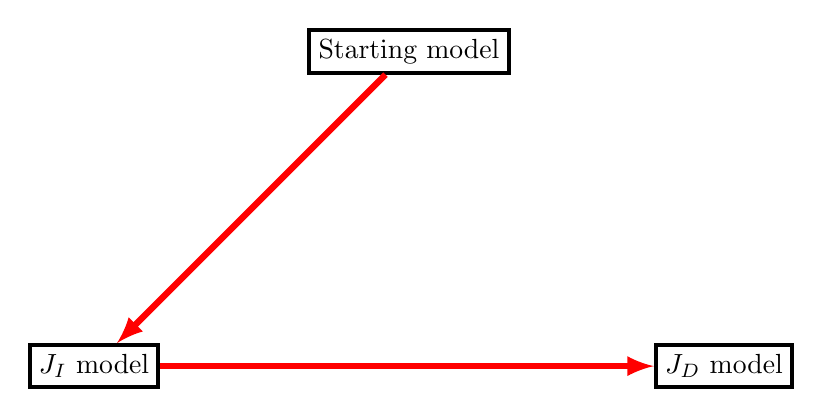
\begin{tikzpicture}
        \path (0,0)  node[RectObject] (x) {Starting model}; 
        \path (4,-4) node[RectObject] (y) {$J_D$ model};
        \path (-4,-4)  node[RectObject] (z) {$J_I$ model};
        \draw[rarrow] (x) -> (z);
        \draw[rarrow] (z) -> (y);
      \end{tikzpicture}
    \end{center}
\end{frame} 

\inputdir{workshop}


\begin{frame}
  \vspace{.63cm}
    \begin{flushleft}
      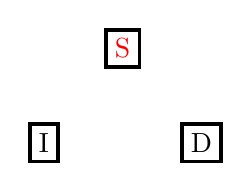
\begin{tikzpicture}
        \path (0,0)  node[RectObject] (x) {{\red S}}; 
        \path (1.,-1.2) node[RectObject] (y) {D};
        \path (-1,-1.2)  node[RectObject] (z) {I};
      \end{tikzpicture}
    \end{flushleft}
  \vspace{-1cm}
 \plot{image-wtomo-cip}{width=\textwidth}{}
\end{frame}




\begin{frame}
  \vspace{.63cm}
    \begin{flushleft}
      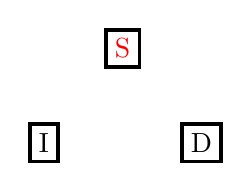
\begin{tikzpicture}
        \path (0,0)  node[RectObject] (x) {{\red S}}; 
        \path (1.,-1.2) node[RectObject] (y) {D};
        \path (-1,-1.2)  node[RectObject] (z) {I};
      \end{tikzpicture}
    \end{flushleft}
  \vspace{-1cm}
 \plot{image-winit}{width=\textwidth}{}
\end{frame}


\begin{frame}
  \vspace{.63cm}
    \begin{flushleft}
      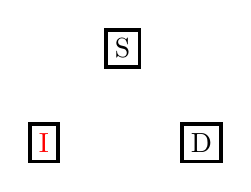
\begin{tikzpicture}
        \path (0,0)  node[RectObject] (x) {S}; 
        \path (1.,-1.2) node[RectObject] (y) {D};
        \path (-1,-1.2)  node[RectObject] (z) {{\red I}};
      \end{tikzpicture}
    \end{flushleft}
  \vspace{-1cm}
 \plot{image-wtomo}{width=\textwidth}{}
\end{frame}

\begin{frame}
  \vspace{.63cm}
    \begin{flushleft}
      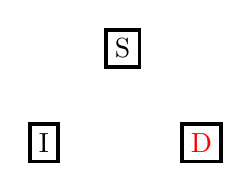
\begin{tikzpicture}
        \path (0,0)  node[RectObject] (x) {S}; 
        \path (1.,-1.2) node[RectObject] (y) {{\red D}};
        \path (-1,-1.2)  node[RectObject] (z) {I};
      \end{tikzpicture}
    \end{flushleft}
  \vspace{-1cm}
 \plot{image-wfwi}{width=\textwidth}{}
\end{frame}





\begin{frame}
  \vspace{.63cm}
    \begin{flushleft}
      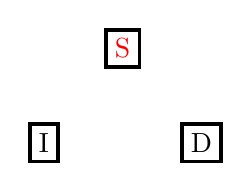
\begin{tikzpicture}
        \path (0,0)  node[RectObject] (x) {\red{S}}; 
        \path (1.,-1.2) node[RectObject] (y) {D};
        \path (-1,-1.2)  node[RectObject] (z) {I};
      \end{tikzpicture}
    \end{flushleft}
  \vspace{-1cm}
 \plot{anglex-image-winit}{width=\textwidth}{}
\end{frame}


\begin{frame}
  \vspace{.63cm}
    \begin{flushleft}
      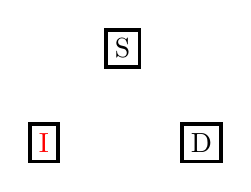
\begin{tikzpicture}
        \path (0,0)  node[RectObject] (x) {S}; 
        \path (1.,-1.2) node[RectObject] (y) {D};
        \path (-1,-1.2)  node[RectObject] (z) {\red{I}};
      \end{tikzpicture}
    \end{flushleft}
  \vspace{-1cm}
 \plot{anglex-image-wtomo}{width=\textwidth}{}
\end{frame}

\begin{frame}
  \vspace{.63cm}
    \begin{flushleft}
      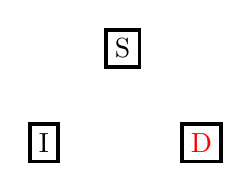
\begin{tikzpicture}
        \path (0,0)  node[RectObject] (x) {S}; 
        \path (1.,-1.2) node[RectObject] (y) {\red{D}};
        \path (-1,-1.2)  node[RectObject] (z) {I};
      \end{tikzpicture}
    \end{flushleft}
  \vspace{-1cm}
 \plot{anglex-image-wfwi}{width=\textwidth}{}
\end{frame}









\begin{frame}
  \vspace{.63cm}
    \begin{flushleft}
      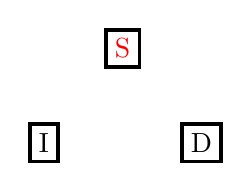
\begin{tikzpicture}
        \path (0,0)  node[RectObject] (x) {\red{S}}; 
        \path (1.,-1.2) node[RectObject] (y) {D};
        \path (-1,-1.2)  node[RectObject] (z) {I};
      \end{tikzpicture}
    \end{flushleft}
  \vspace{-1cm}
 \plot{vel-winit}{width=\textwidth}{}
\end{frame}


\begin{frame}
  \vspace{.63cm}
    \begin{flushleft}
      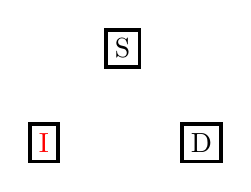
\begin{tikzpicture}
        \path (0,0)  node[RectObject] (x) {S}; 
        \path (1.,-1.2) node[RectObject] (y) {D};
        \path (-1,-1.2)  node[RectObject] (z) {\red{I}};
      \end{tikzpicture}
    \end{flushleft}
  \vspace{-1cm}
 \plot{vel-wtomo}{width=\textwidth}{}
\end{frame}

\begin{frame}
  \vspace{.63cm}
    \begin{flushleft}
      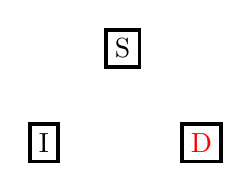
\begin{tikzpicture}
        \path (0,0)  node[RectObject] (x) {S}; 
        \path (1.,-1.2) node[RectObject] (y) {\red{D}};
        \path (-1,-1.2)  node[RectObject] (z) {I};
      \end{tikzpicture}
    \end{flushleft}
  \vspace{-1cm}
 \plot{vel-wfwi}{width=\textwidth}{}
\end{frame}

\begin{frame}
\end{frame}



\begin{frame}\frametitle{conclusions}
  \begin{columns}
    \column{0.5\textwidth}
      \itab{cost}
    \column{0.5\textwidth}
      \itab{CIP}
  \end{columns}
  \vfill
  \pause
  \begin{columns}
    \column{0.5\textwidth}
      \itab{illumination}
    \column{0.5\textwidth}
      \itab{PSF penalty}
  \end{columns}
  \vfill
  \pause
  \begin{columns}
    \column{0.5\textwidth}
      \itab{resolution}
    \column{0.5\textwidth}
      \itab{data-domain WT}
  \end{columns}
  \vfill
\end{frame}


\begin{frame}\frametitle{acknowledgments}
\cen{Bruce VerWest, Gerhard Pratt, Yuting Duan, Tariq Alkhalifah, and Zedong Wu.}
\end{frame}

\begin{frame}\frametitle{acknowledgments}
\begin{figure}[p]
    \includegraphics[width=0.3\textwidth]{cgg}
\end{figure}
\end{frame}

\inputdir{.}
\begin{frame}\frametitle{acknowledgments}
  \plot{thank2}{height=.9\textheight}{}
\end{frame}


\begin{frame}
\end{frame}

